%%%%%%%%%%%%%%%%%%%%%%%%%%%%%%%%%%%%%%%%%%%%%%%%%%%%%%%%%%%%%%%%%%%%%%%%%%%%%%%%%%%%%%%%%%%%%%%%%%%%%%%%%%%%
%%%%%%%%%%%%%%%%%%%%%%%%%%%%%%%%%% RESULTS   
%%%%%%%%%%%%%%%%%%%%%%%%%%%%%%%%%%%%%%%%%%%%%%%%%%%%%%%%%%%%%%%%%
%%%%%%%%%%%%%%%%%%%%%%%%%%%%%%%%%%%%%%%%%%%%%%%%%%%%%%%%%%%%%%%%%%%%%%%%%%%%%%%%%%%%%%%%%%%%%%%%%%%%%%%%%%%%

\section{Results} \label{sec:results}

An increase of one unit in $IVUR$ signifies the addition of as many new job openings in a district as there were unemployed individuals, while maintaining the unemployment count steady. Meanwhile, a one-unit increase in the $IPBL$ represents an increase in potential benefit levels by €1,000. To obtain easy-to-interpret effect sizes, we use a shift roughly amounting to the standard deviation (s.d.) and the interquartile range of the $IVUR$ and $IPBL$ as a reference. For the $IVUR$, this shift denotes an increment of 0.2 ($s.d.=0.153, IQR=0.211$), and for the $IPBL,$  an increase of 0.3 (€300, $s.d.=316.9, IQR=456$).\footnote{We use round numbers in the ballpark of the standard deviation and the IQR for ease of interpretation.} Subsequently, we term this a \textit{standard shift} or a \textit{standard increase}.
Multiplying the shift with $\beta_{1,t}$ for the $IVUR$ and $\beta_{2,t}$ for the $IPBL$ gives us the change in the outcome for each respective increase.

\subsection{Effects on labor market outcomes}
 %and internal mobility

Figure~\ref{fig:economic_results} presents the primary results for selected labor market outcomes. Panels (a) through (d) illustrate how an increase of one unit in $IVUR$ or $IPBL$ impacts (a) the likelihood of being in employment, (b) the unconditional monthly real earnings (in 2015 euro), (c) the log of real monthly wage income (conditional upon employment), and (d) the likelihood of being in marginal employment.

A standard shift in the $IVUR$ increases the employment probability in the $12^{th}$ month after receiving protection by 4 pp. The effect occurs almost immediately after receiving protection and starts to weaken after 18 months, turning zero in month 30. This finding is qualitatively in line with other results in the literature that study the effect of economic conditions at labor market entry on employment outcomes.\footnote{For example, \citet{barsbai2024} find that family migrants who face a higher unemployment rate at immigration are initially less likely to be employed, with the effect disappearing after four years.} Relative to the mean employment rate of 11.3\% in month twelve, a standard increase for $IVUR$ increases the employment probability by 35\%.

Before turning to the $IPBL$ result, recall that $IPBL$ measures the potential cash benefit: the coefficient pools refugees in private accommodation (directly exposed) and in organized accommodation (only indirectly exposed via the option of moving to private accommodation), and should therefore be read as a diluted average effect (see Section~\ref{sec:discussion}). A standard increase in the $IPBL$ decreases the employment probability by 1.51 pp. in month twelve (13.3\% of the mean). This effect also disappears after 30 months.

Panel (b) shows the effects on monthly earnings. The patterns of the effects closely follow the employment effect. A standard shift in the $IVUR$ increases earnings by €81 (39\% relative to the mean in month twelve), and a standard shift in $IPBL$, decreases earnings by €33 (-15.8\% relative to the mean in month twelve), in monthly real earnings. Another way to interpret the effect of $IPBL$ is that every €100 increase in potential benefits results in a decrease of €11 in monthly real earnings.

The similarity of the patterns in Panels (a) and (b) strongly suggests that changes in employment drive the effects on earnings. To understand whether the shocks also affect wages, we use log real monthly wage income (conditional on having any income) as an outcome in Panel (c).\footnote{This analysis on wage income is conditional on being employed and rests on the assumption that sorting into employment is unrelated to $IVUR$ and $IPBL$.} We do not find any statistically significant effects on wages, contrasting other findings in the literature of rather persistent wage effects \citep{barsbai2024}. Panel (d) suggests a tiny positive effect of a higher $IVUR$ on the likelihood of marginal employment starting after twelve months, with the $IPBL$ showing no discernible effect.

\begin{figure}
    \caption{Effect of the $IVUR$ and $IPBL$ on selected labor market outcomes}
    \label{fig:economic_results}
    \begin{center}
    \vspace{-0.5 cm}
    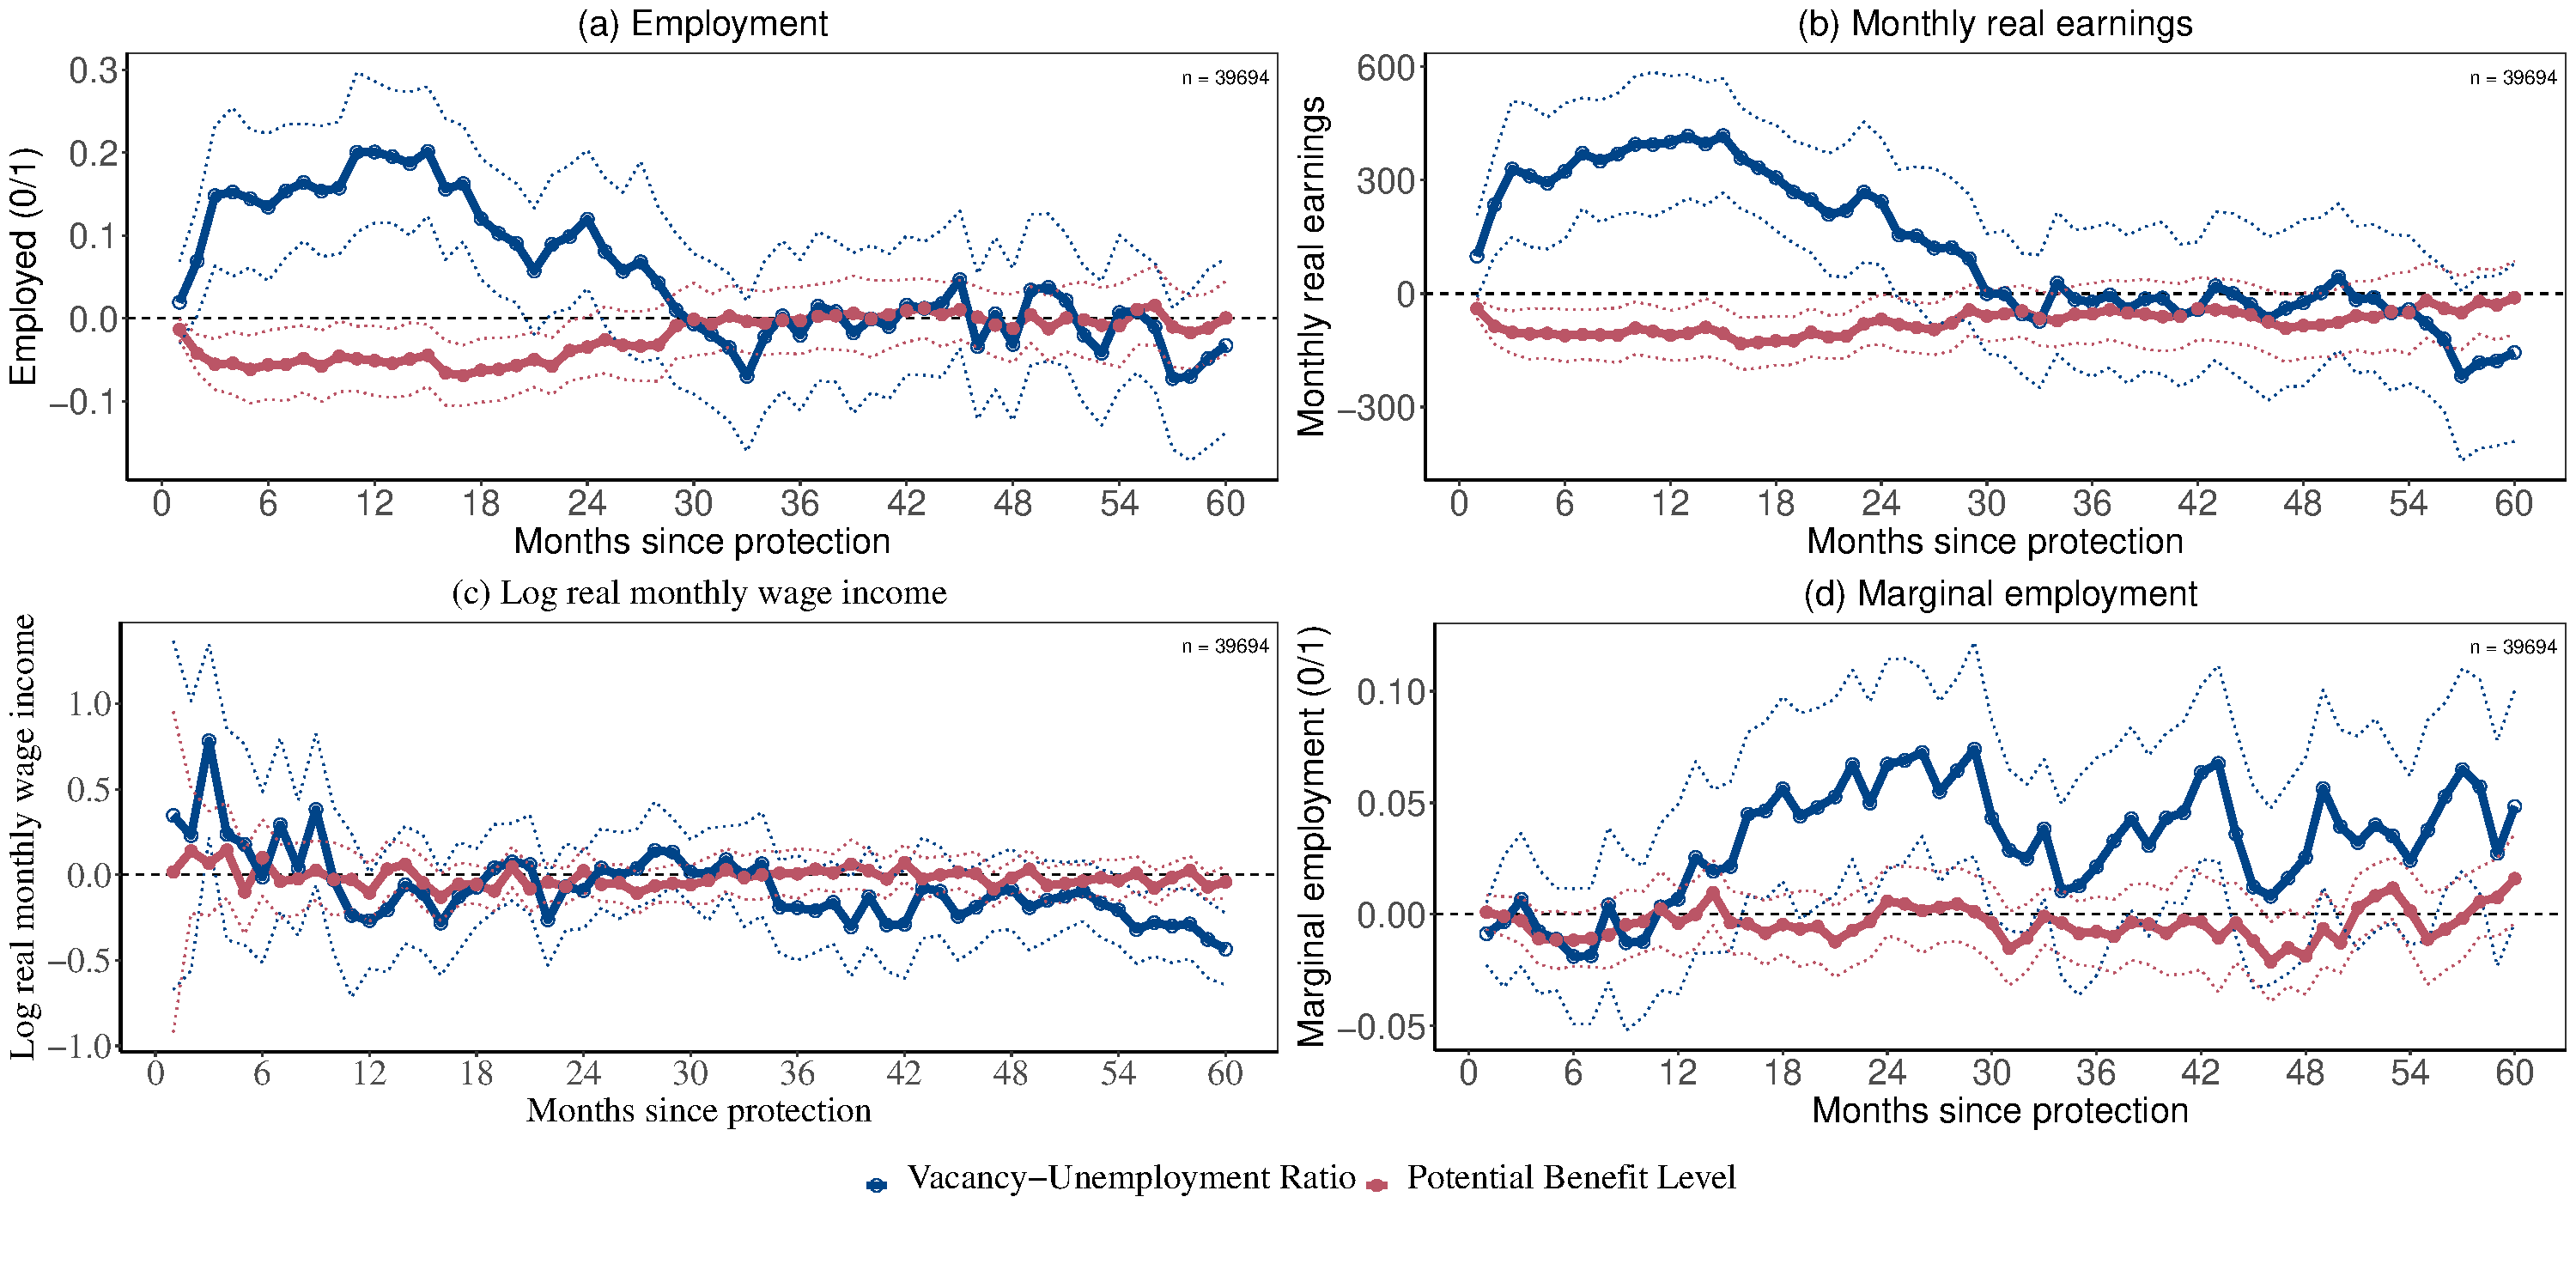
\includegraphics[scale=0.31]{figures/fig_employment_income.pdf}
    \end{center}
    \vspace{-0.5 cm}
    \fignote{\footnotesize \textit{Notes:} The x-axis shows the months since protection was received. The y-axis displays the effect of a one-unit increase in either i) the vacancy-to-unemployment ratio or ii) the potential benefit level, measured in €1,000 (real 2015 values), on selected outcomes. The panels show the effects on (a) having any type of part- or full-time employment (binary); panel (b) the unconditional monthly real earnings (in 2015 euro); panel (c) the log real monthly wage income (conditional on being employed); and panel (d) the probability of having a mini-job (below €406 in 2015). All regressions include a full set of arrival-group, year-month, and district-of-protection fixed effects. Additional control variables include age and age squared at immigration, gender, type of protection, family status at protection date, and country of origin. Standard errors are clustered at the state-year-of-protection level. Dashed lines indicate 95\% confidence intervals.}
\end{figure}

\FloatBarrier


\subsection{Effects on internal mobility}
 
Better labor market conditions and higher benefits should reduce the likelihood of relocating, which is very common among refugees after receiving protection (see Figure \ref{fig:descriptive_outcomes_main}). We show results for mobility in Figure~\ref{fig:mobility_results}. 

In Panel (a), we observe that an increase in the $IVUR$ has a statistically significant positive impact on the likelihood of refugees staying in the state. Specifically, a standard shift in the $IVUR$ leads to a 3.9 pp. increase in this probability in month twelve. Similarly, a standard shift in the $IPBL$ results in a 2.8 pp. increase in the same likelihood in month twelve. The effects become somewhat weaker over time but persist for 60 months, suggesting that enhanced welfare benefits and a strong labor market both positively influence the likelihood of refugees staying in their original state.

These findings are further supported by the observations in panel (b). Here, we note a consistent negative effect of the $IPBL$ on the likelihood of relocating to Vienna for those not initially assigned to Vienna. The $IVUR$  also has a negative but not persistent and only marginally significant effect.

The similarity of approaches allows for a direct comparison with the results of \citet{ferwerda2023}, who study the effect of current benefit levels on the probability of immigrants moving within Switzerland. They find that increasing benefits from less than 750 CHF to 751-1500 CHF increases the likelihood of staying by about 1.5 pp. while an increase to 1500-3000 CHF increases it by about 2 pp. Our effects are significantly larger, as a 2 pp. change in the probability is triggered by a roughly €200 change in benefit levels. A likely explanation is that the effects in the Austrian context are larger because the treatment is applied when refugees receive protection, when they are not yet strongly tied to a specific location and are potentially more mobile.\footnote{Alternatively, we can approximate an elasticity of the mover rate with respect to benefit levels. However, providing a single elasticity is difficult, as the result depends on the point of evaluation, i.e.\ which benefit level is 
considered (which varies substantially across states) and which mover rate is taken as the baseline. As an example, take Upper Austria.  The mean mover rate is 0.29. The reform reduced benefits from roughly €1,000 to €700 (incl. housing benefits), and we estimate that a €100 reduction increases the mover rate by roughly one pp. Evaluating the elasticity at the midpoint 
benefit level of €850 and an implied mover rate of 0.29, the percentage change in benefits is $-100/850 \approx -11.8\%$ while the corresponding change in the mover rate is $0.01/0.29 \approx 3.4\%$.
This yields an elasticity of $3.4/11.8 \approx 0.29$.}

\begin{figure}
    \caption{Effect of the $IVUR$ and $IPBL$ on mobility outcomes}
    \label{fig:mobility_results}
    \begin{center}
    \vspace{-0.5 cm}
    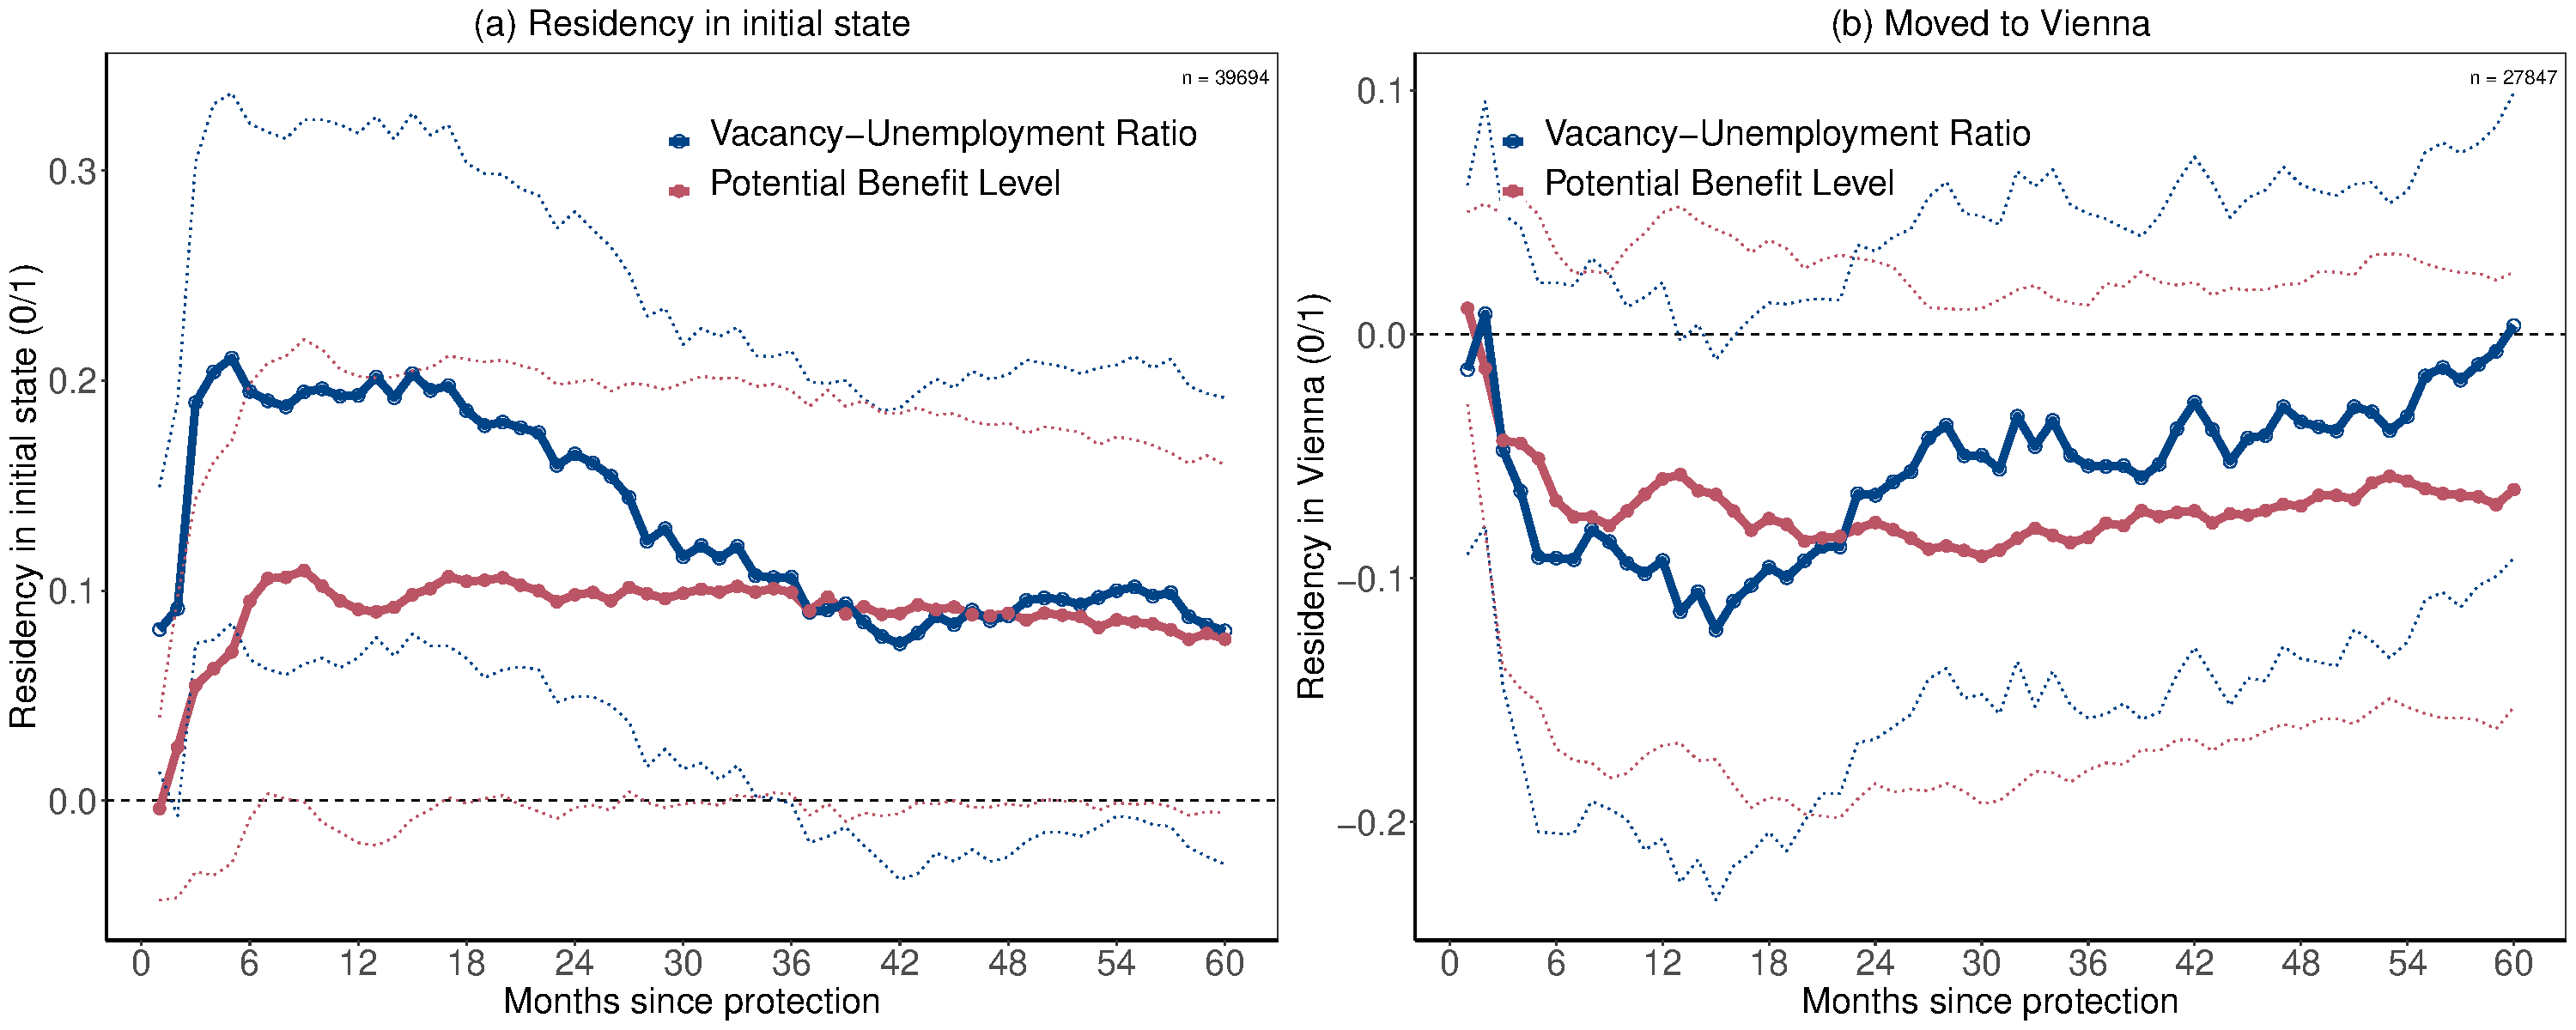
\includegraphics[scale=0.31]{figures/fig_mobility.pdf}
    \end{center}
    \fignote{\footnotesize \textit{Notes:} The x-axis shows the months since protection was received. The y-axis displays the effect of a one-unit increase in either i) the vacancy-to-unemployment ratio or ii) the potential benefit level, measured in €1,000 (real 2015 values), on selected outcomes. Panel (a) shows the effects on the probability of living in the state of protection; panel (b) shows the effect on moving to Vienna (conditional on residing outside Vienna at the time of protection). All regressions include a full set of arrival-group, year-month, and district-of-protection fixed effects. Additional control variables include age and age squared at immigration, gender, type of protection, family status at protection date, and country of origin. Standard errors are clustered at the state-year-of-protection level. Dashed lines indicate 95\% confidence intervals.}
\end{figure}

In Figure~\ref{fig:empl_reloc}, we show how the effects on employment and location choice interplay. A higher $IVUR$ positively affects the joint probability of being employed and in the initial state (panel (a)) and negatively affects the joint probability of being not employed and in another state (panel (d)). In other words, migrants stay because they are in employment instead of moving and needing to search for a job in another state. 

\begin{figure}
    \caption{Effect of the $IVUR$ and $IPBL$ on employment and location choice}
    \label{fig:empl_reloc}
    \begin{center}
    \vspace{-0.5 cm}
    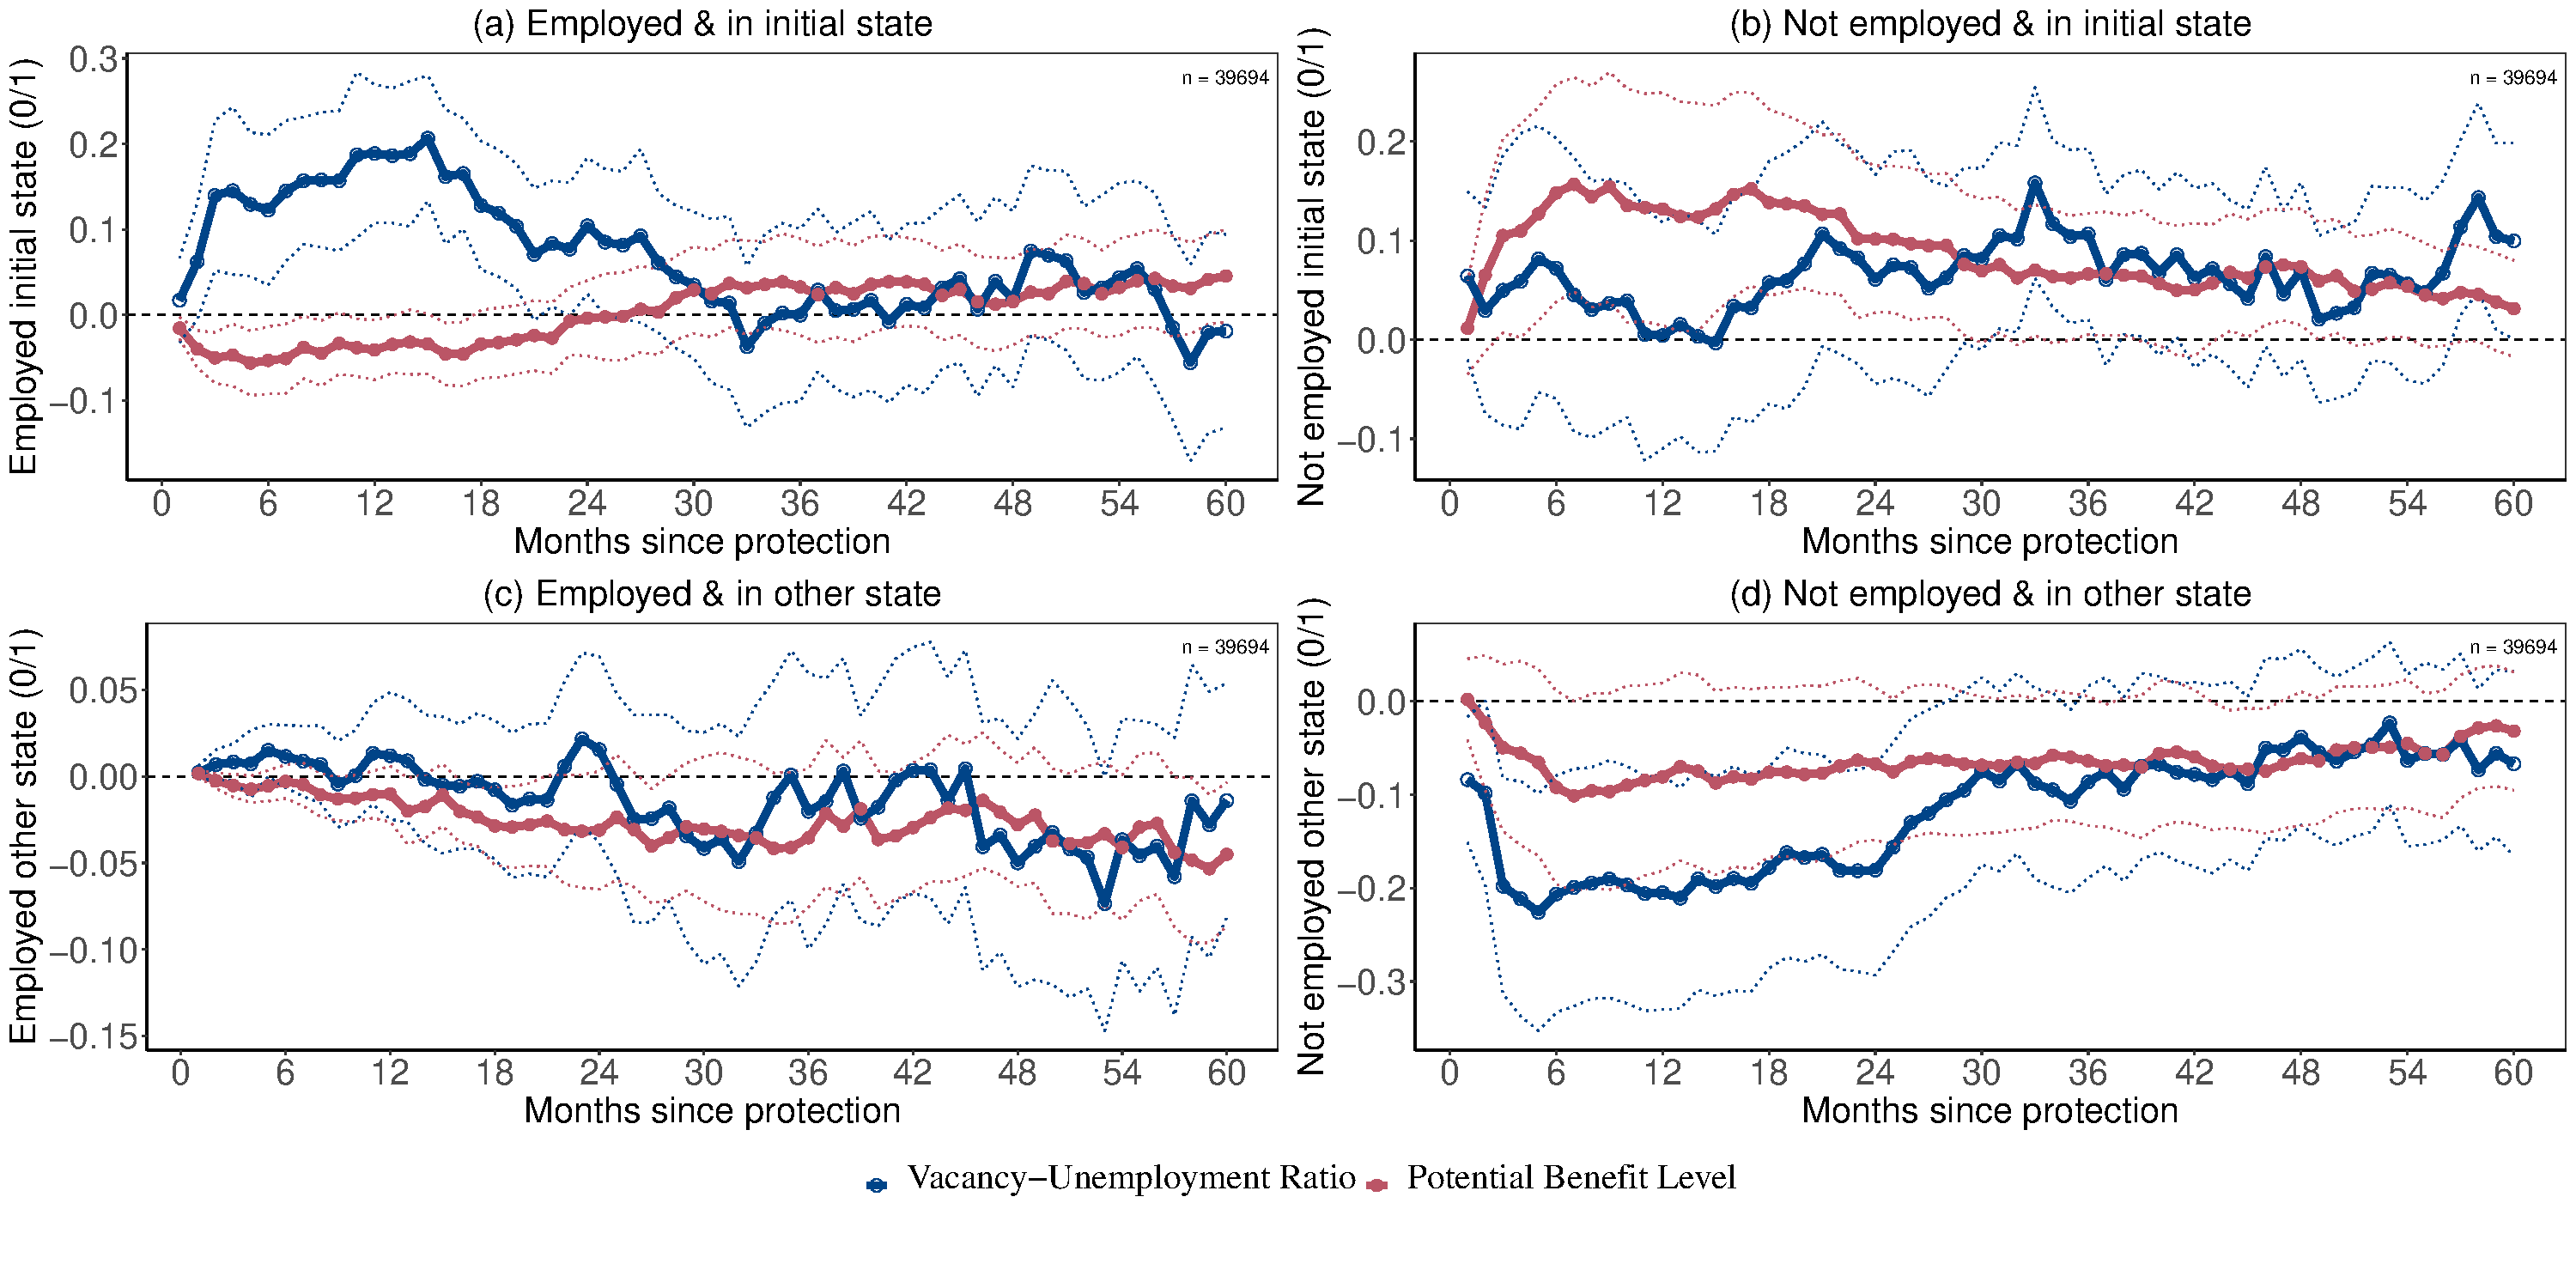
\includegraphics[scale=0.31]{figures/fig_employment_relocation.pdf}
    \end{center}
    \fignote{\footnotesize \textit{Notes:} The x-axis shows the months since protection was received. The y-axis displays the effect of a one-unit increase in either i) the vacancy-to-unemployment ratio or ii) the potential benefit level, measured in €1,000 (real 2015 values), on selected outcomes. Panel (a) shows the effects on the joint probability of being employed and living in the initial state; panel (b) shows the effect on the joint probability of being not employed and living in the initial state. Panel (c) shows the effects on the joint probability of being employed and living in another state; panel (d) shows the effect on the joint probability of not being employed and living in another state. All regressions include a full set of arrival-group, year-month, and district-of-protection fixed effects. Additional control variables include age and age squared at immigration, gender, type of protection, family status at protection date, and country of origin. Standard errors are clustered at the state-year-of-protection level. Dashed lines indicate 95\% confidence intervals.}
\end{figure}

In contrast, the $IPBL$ has a stronger effect on the joint probability of being not employed and in the initial state (panel (b)). However, this is primarily due to a higher likelihood of remaining in the state, rather than to changing employment prospects. This becomes apparent from the negative effect on not being employed and in another state (panel (d)).

This suggests that strong labor markets increase the probability that individuals remain in their initial state, owing to job availability. In contrast, weak labor markets might incentivize relocation to another state without prospects of work in the destination state. Additionally, these findings indicate that benefit levels are relevant for the location choice but less so for employment trajectories.

\FloatBarrier

\subsection{Effects on receiving social support}

The third group of outcomes consists of measures of social support receipt. Figure~\ref{fig:welfare_results} shows the effects on the likelihood of (a) utilizing services from the public employment service and (b) receiving welfare benefits.

We do not observe any effect of the $IVUR$ or $IPBL$ on utilizing PES services (Panel (a)). If anything, a higher $IPBL$ has a small negative effect in the first nine months.

%Nevertheless, the zero average effect might mask two cont Individuals who do not receive support might either have secured regular employment, negating the need for further support services, or might be lacking such services due to underperformance. These contrasting scenarios could neutralize each other, resulting in the observed insignificance.

Panel (b) shows a significant negative impact of the $IVUR$ on the probability of receiving welfare benefits in the first 30 months. Interestingly, the magnitude of this effect is consistent with the positive effect of the $IVUR$ on employment (Figure \ref{fig:economic_results}, Panel (a)). Furthermore, the impact on receiving welfare benefits diminishes and becomes statistically insignificant after 30 months, mirroring the trajectory of the employment effect. This suggests that refugees who secure employment due to favorable local labor market conditions are less likely to rely on welfare benefits.

Similarly, we observe that a higher $IPBL$ has a small but significant effect on the likelihood of receiving welfare benefits, particularly in the years 2 and 3 after receiving protection. The effect is largest about 24 months after receiving protection, when a standard shift in $IPBL$ increases the probability of receiving welfare benefits by about 2.5 pp. Again, the pattern mirrors the effect of $IPBL$ on employment.

%A shift in the $IVUR$ from the first to the third quartile reduces the likelihood of receiving welfare benefits by 4.9 percentage points, relative to a base rate of 76.1\% of refugees obtaining welfare benefits in month 12.

\begin{figure}
    \caption{Effect of the $IVUR$ and $IPBL$ on selected social support outcomes}
    \label{fig:welfare_results}
    \begin{center}
    \vspace{-0.5 cm}
    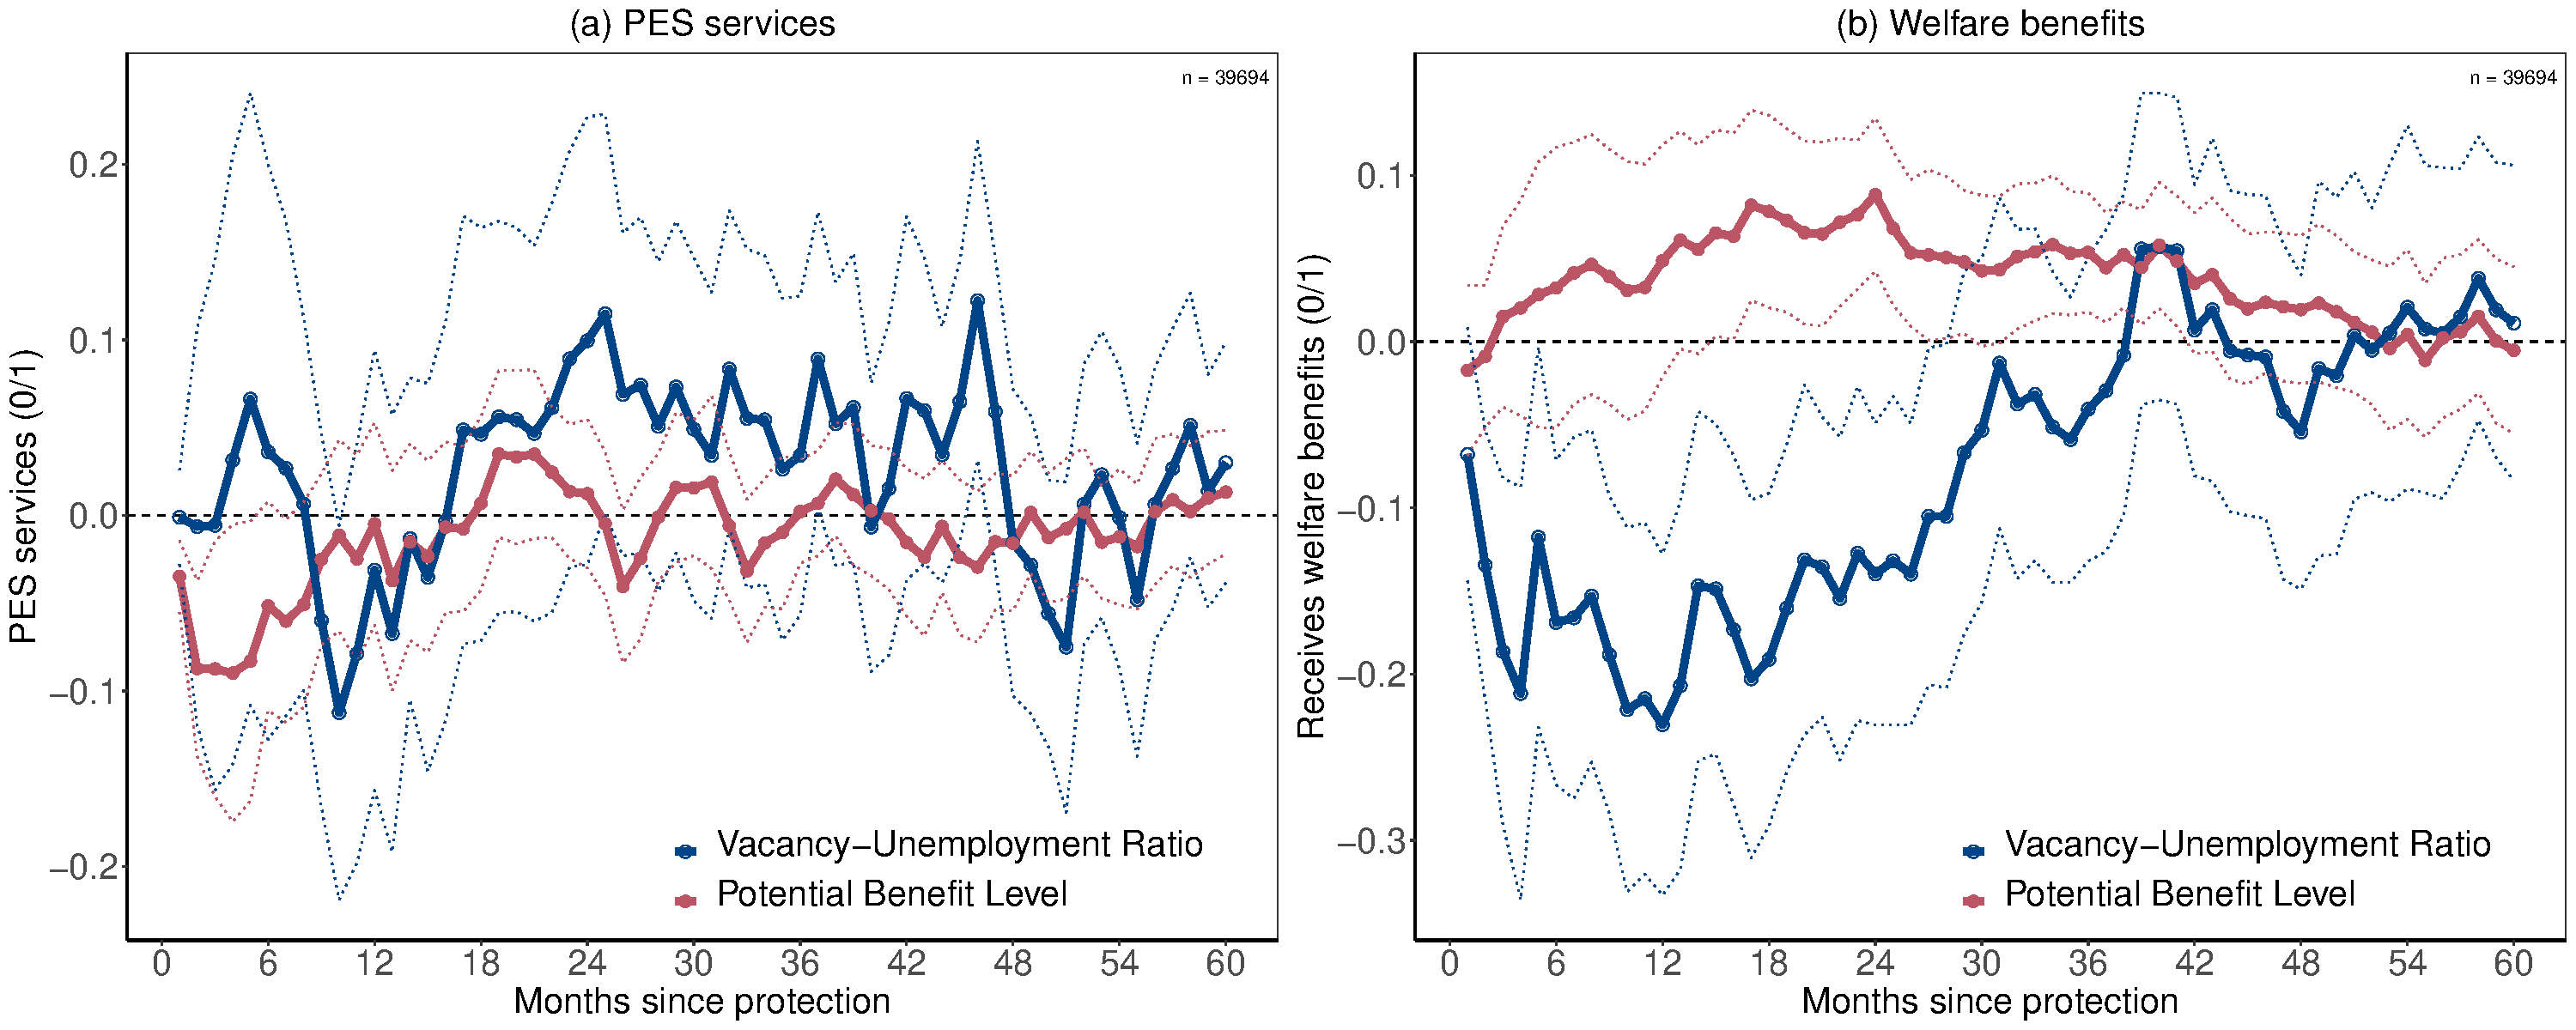
\includegraphics[scale=0.31]{figures/fig_social_support.pdf}
    \end{center}
    \fignote{\footnotesize \textit{Notes:} The x-axis shows the months since protection was received. The y-axis displays the effect of a one-unit increase in either i) the vacancy-to-unemployment ratio or ii) the potential benefit level, measured in €1,000 (real 2015 values), on selected outcomes. The panels show the effects on (a) the probability of making use of PES services and (b) the probability of receiving welfare benefits. All regressions include a full set of fixed effects for arrival group, year-month, and district of protection. Additional control variables include age and age squared at immigration, gender, type of protection, family status at protection date, and country of origin. Standard errors are clustered at the state-year-of-protection level. Dashed lines indicate 95\% confidence intervals.}
\end{figure}

\FloatBarrier




\subsection{Interplay of labor market tightness and benefit levels}

Our main specification, as presented in Equation \ref{eq:main}, estimates how $IVUR$ and $IPBL$ independently affect refugees' economic and social integration after receiving protection. To further explore the relationships between these variables, we introduce an interaction term between $IVUR$ and $IPBL$ in Equation \ref{eq:main_interaction}:

A negative cross-partial of $IVUR$ and $IPBL$ on employment is consistent with a standard equilibrium search framework \citep{pissarides2000}, in which higher labor market tightness raises the offer arrival rate, so the disincentive effect of a higher reservation wage from more generous benefits binds more tightly when offers are plentiful. \citet{schmieder2016} document the same cross-partial empirically for unemployment insurance across varying labor market conditions.

\begin{equation}\label{eq:main_interaction}
\begin{aligned}
Y_{i,t} = & \, \alpha_t + \beta_{1,t} IVUR_{d_0,t_0} + \beta_{2,t} IPBL_{f,p,s_0,t_0} + \beta_{3,t} IVUR_{d_0,t_0} \times IPBL_{f,p,s_0,t_0} \\
& + \gamma_{t_0} + \delta_{g} + \eta_{d_0} + X_{i}\Delta_t + \epsilon_{i,t},
\end{aligned}
\end{equation}

This specification allows us to calculate and interpret the effects of changes in the $IPBL$ for different levels of labor market tightness.

Table \ref{tab:interactions} reports the results for selected outcomes twelve months after receiving protection. For ease of interpretation, we demeaned $IVUR$ and $IPBL$. The coefficients for the main effects remain comparable to our previous results in direction, magnitude, and statistical significance. The interaction term has a significant, opposing effect on the probability of being in employment and receiving welfare benefits (columns (1) and (4), respectively). For the probability of remaining in the initial state in column (2), we find no statistically significant effect of the interaction, but we find a positive and significant effect on the probability of receiving assistance by the PES in column (3).

The marginal effects are calculated for the $IPBL$. Therefore, we fix the $IVUR$ at zero on the first row, the mean in the second row and at 0.2 above the mean in the third row.

Column (1) shows the effect of changes in benefit levels on the probability of being employed at different levels of labor market tightness. As predicted by the search framework above, changes in benefit levels have practically no effect on the employment probability when the labor market is slack. However, benefit levels affect employment probability strongly when the labor market is tight. We see the inverse effects for the receipt of welfare benefits (column (4)).
These results are in line with both the search prediction and the empirical findings of \citet{dustmann2024}, who find that cuts in welfare benefits in Denmark only affect the employment probability in strong labor markets.

Column (3) suggests that when the labor market is tight, increasing benefits increases the likelihood of receiving assistance from the PES. This is potentially due to the combination of the incentives for public agencies to fill the labor demand, but also to reduce the fiscal cost due to high benefit levels.

\begin{table}
	\caption{Effects of $IVUR$ and $IPBL$ with interactions of treatment variables and marginal effects of $IPBL$ for different levels of $IVUR$, twelve months after protection}
	\label{tab:interactions}
	\begin{threeparttable}
		\begin{small}
			\begin{tabular}{lcccc}				\centering
\begin{tabular}{lcccc}
\hline
& (1) & (2) & (3) & (4) \\
& In employment & In initial state & PES support & Welfare benefits \\ 
\hline
\textbf{Coefficients} \\
IVUR & 0.188*** & 0.189** & -0.021 & -0.218*** \\
& (0.044) & (0.062) & (0.056) & (0.048) \\ 
IPBL & -0.050** & 0.091** & -0.005 & 0.048* \\
& (0.018) & (0.030) & (0.025) & (0.024) \\ 
IVUR:IPBL & -0.294*** & -0.091 & 0.230*** & 0.280*** \\
& (0.043) & (0.112) & (0.055) & (0.071) \\ 
\hline
\textbf{Marginal Effects} \\
IPBL (IVUR=0) & 0.006 & 0.108 & -0.049 & -0.006 \\
IPBL (IVUR=0.192) & -0.050 & 0.091 & -0.005 & 0.048 \\
IPBL (IVUR=0.392) & -0.109 & 0.073 & 0.041 & 0.104 \\
\hline
\end{tabular}
			\end{tabular}
		\end{small}
		\begin{tablenotes} 
			\begin{footnotesize}
				\begin{spacing}{1}
					\textit{Notes:} The upper part of the table reports OLS estimates for $IVUR$, $IPBL$ and their interaction. The lower part reports marginal effects for $IPBL$, fixing $IVUR$ at zero, the mean (0.192) or 0.2 above the mean. The column title shows the outcome variable. All regressions include a full set of arrival-group, year-month, and district-of-protection fixed effects. Additional control variables include age and age squared at immigration, gender, type of protection, family status at protection date, and country of origin. Standard errors are clustered at the state-year-of-protection level. */**/*** denote statistical significance at the 10/5/1 percent level.
				\end{spacing}
			\end{footnotesize}
		\end{tablenotes}
	\end{threeparttable}
\end{table}


\FloatBarrier

\subsection{Effect heterogeneity by gender}

One notable observation is the significant disparity in labor market integration between genders, with women's employment rates at only 20\% even five years post-protection, in stark contrast to men's, which is 60\% (see Figure \ref{fig:descriptive_outcomes_main}).

In this section, we investigate whether men and women also differ in their reactions to $IVUR$ and $IPBL$.  For this, we conduct the analysis separately for men and women with the results shown in Figure \ref{fig:gender}. 

\begin{figure}
    \caption{Effect heterogeneity by gender}
    \label{fig:gender}
    \begin{center}
    \vspace{-0.5 cm}
    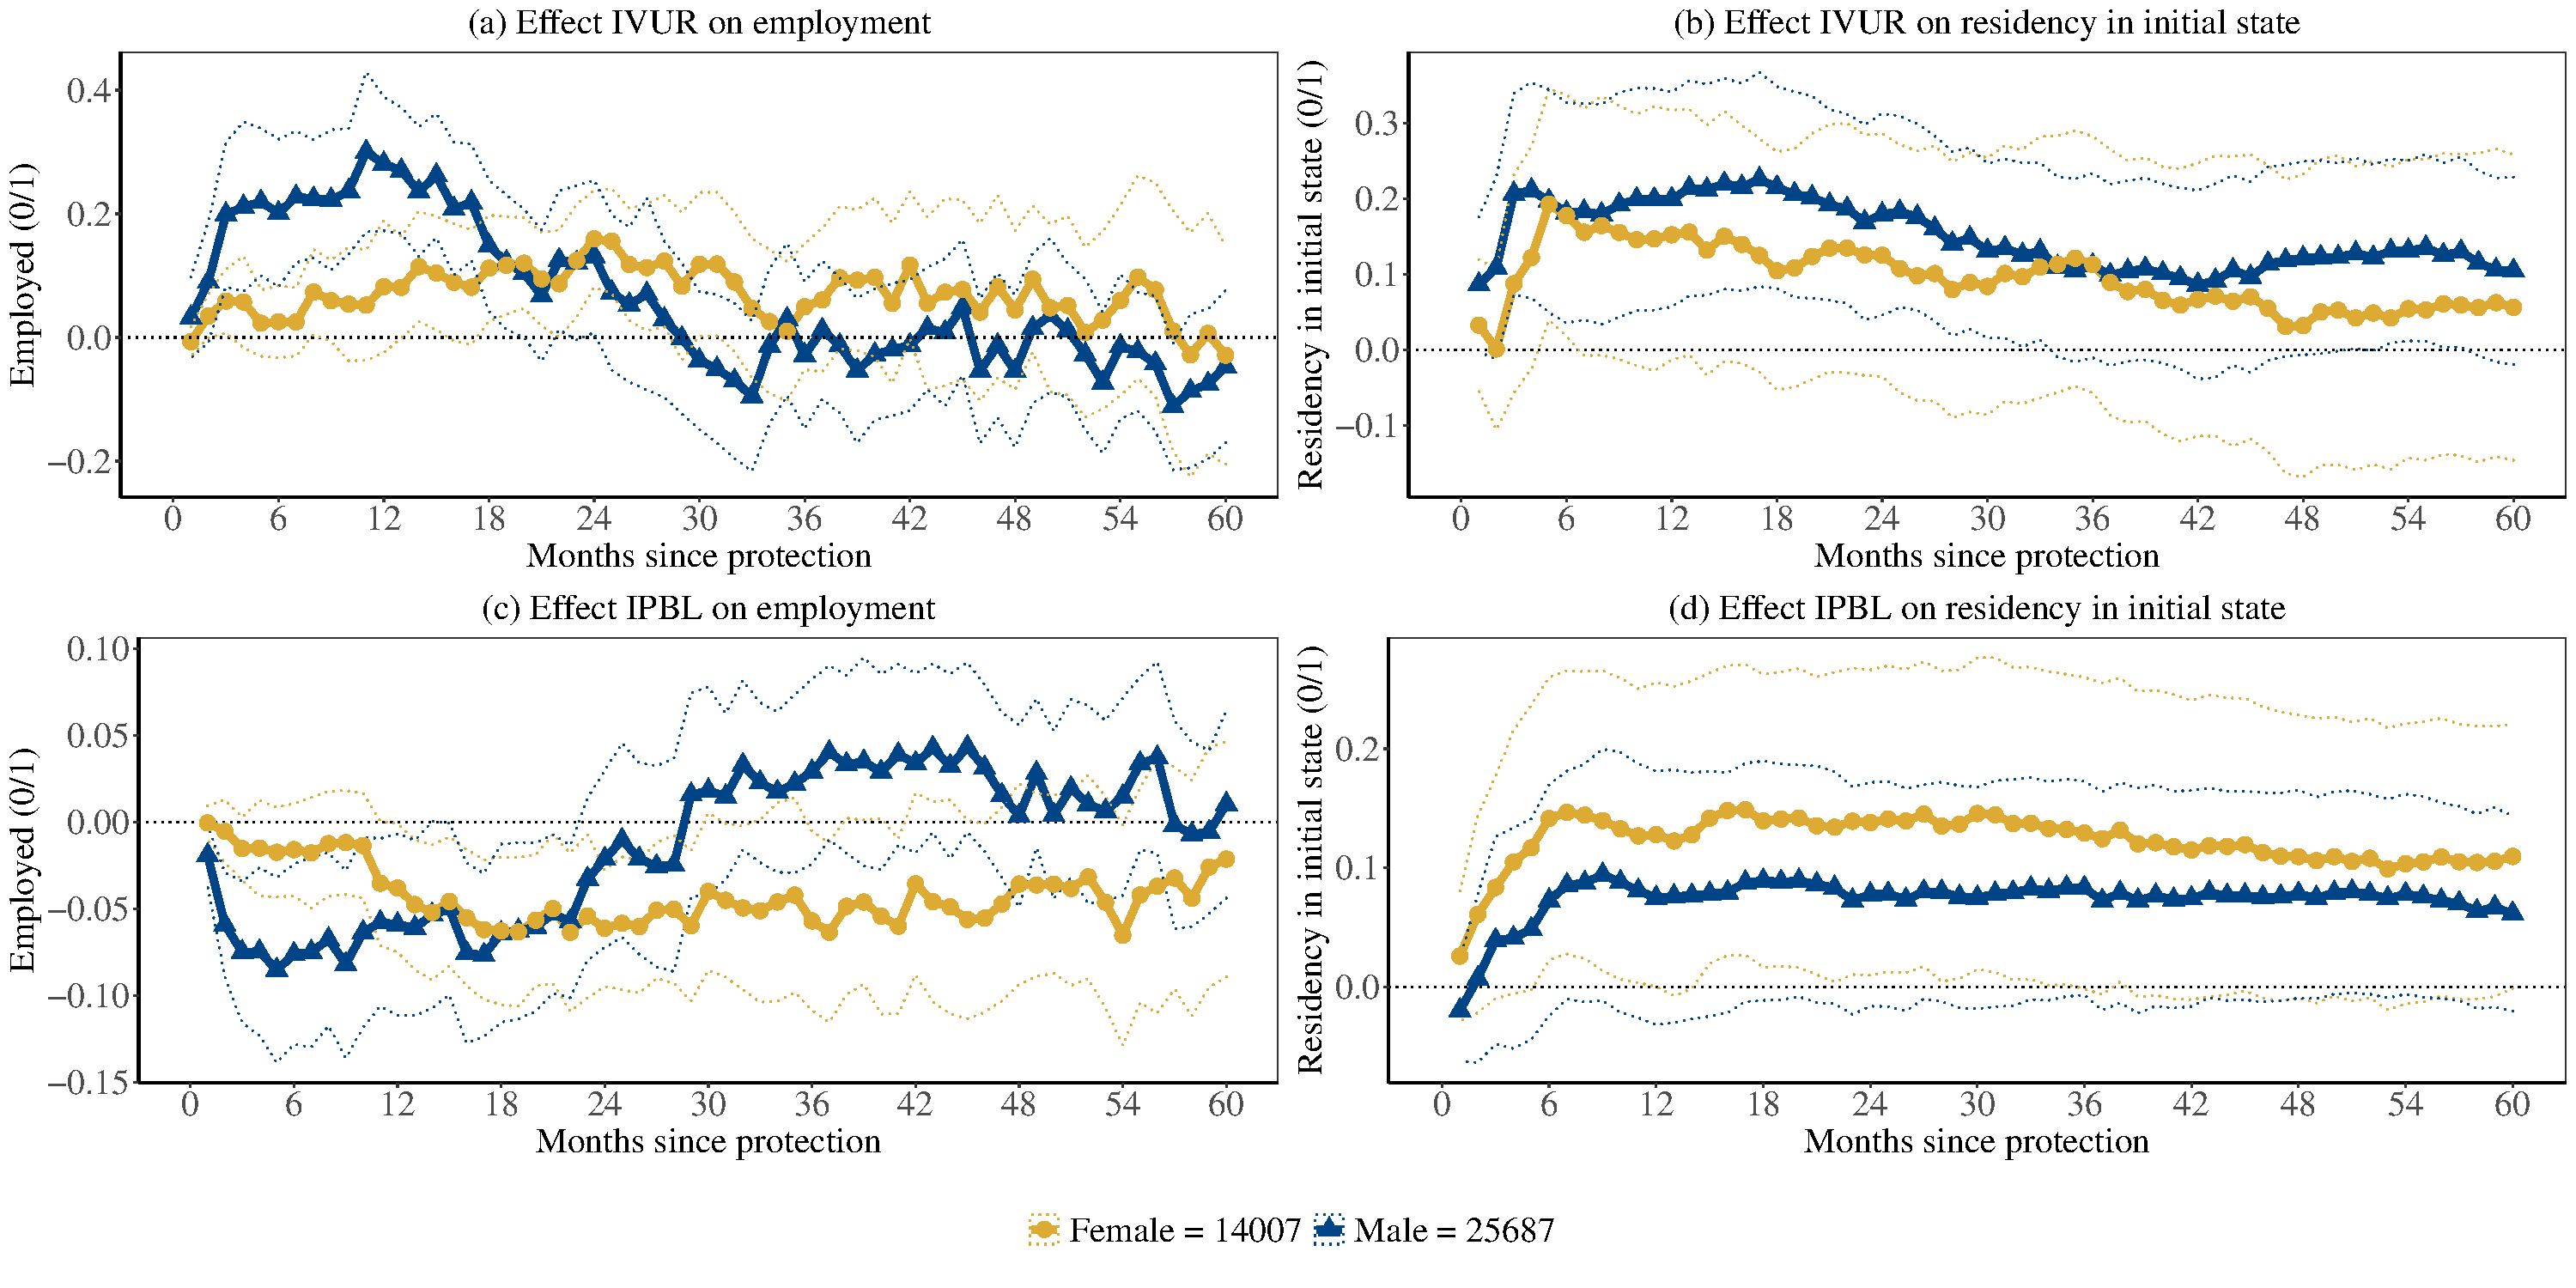
\includegraphics[scale=0.31]{figures/fig_gender.pdf}
    \end{center}
    \vspace{-0.5em}
\fignote{\footnotesize \textit{Notes:} The x-axis shows the months since protection was received. The y-axis displays the effect of a one-unit increase in either (i) the vacancy-to-unemployment ratio or (ii) the potential benefit level, measured in €1,000 (real 2015 values), on selected outcomes. Panels (a) and (b) show the effects of $IVUR$ on employment and on the probability of staying in the initial state, respectively. Panels (c) and (d) show the effects of $IPBL$ on employment and on the probability of staying in the initial state, respectively. Estimates are shown separately for men and women. All regressions include a full set of arrival-group, year-month, and district-of-protection fixed effects. Additional control variables include age and age squared at immigration, type of protection, family status at protection date, and country of origin. Standard errors are clustered at the state-year-of-protection level. Dashed lines indicate 95\% confidence intervals.}
\end{figure}

Panel (a) shows the effects of $IVUR$ on employment. $IVUR$ strongly affects the employment probability of men in the first 18 months after protection, but has hardly any effect on women. Still, for women, we do see some positive effects from around month twelve onwards. While this effect is small in absolute terms, it is not in relative terms, given the extremely low employment rate of female refugees. Panel (b) shows the effect of $IVUR$ on mobility. Point estimates are slightly larger for men, but overall, the pattern is similar. Panel (c) shows the effect of $IPBL$ on employment. While men initially reduce their employment more in response to higher benefits, the effect persists only for 30 months. For women, the negative effect of $IPBL$ on employment is small but relatively persistent. Finally, Panel (d) shows that the effect of $IPBL$ on the likelihood of staying in the state is somewhat stronger for women and persistent for both groups. 

These findings align with the behavior predicted by traditional household models. When men primarily engage in market activities and actively seek employment, their sensitivity to labor market tightness is expected to be higher. For women, labor market tightness is less influential. Regarding mobility, labor market tightness indirectly affects the non-working partner's decisions, especially if the household relocates due to the male partner's unfavorable labor market conditions. Conversely, as men's attachment to the labor market strengthens over time, the significance of benefit levels wanes. However, benefits continue to play a crucial role for women, significantly influencing location choices within Austria.


\subsection{Relevant initial labor market}
As noted by \citet{aslund_when_2007}, it is not clear at what point in time initial local labor market conditions should be measured for refugees. While most of the literature focuses on labor market conditions at the time of immigration, institutional factors limit refugees' labor market access until they have been granted protection (12 months after arrival in our sample). 

Hence, to compare our results to the standard specification in the literature, we add $IVUR$ and $IPBL$ measured at the time of immigration to our regressions. Table \ref{tab:ivuripbl_arrival} shows the results for two outcomes, employment and residency in the initial state, for month 12 after receiving protection.

\begin{table}
  \centering
  \caption{Effects of IVUR and IPBL at Approval on Employment and Residency \\* controlling for IVUR and IPBL at Arrival}
  \label{tab:ivuripbl_arrival}
  \begin{talltblr}[         %% tabularray outer open
entry=none,label=none,
note{}={},
]                     %% tabularray outer close
{                     %% tabularray inner open
colspec={Q[]Q[]Q[]},
column{1}={halign=l,},
column{2}={halign=c,},
column{3}={halign=c,},
}                     %% tabularray inner close
\toprule
& Employed & Residency in initial state \\ \midrule %% TinyTableHeader
IVUR at approval & \num{0.195}*** & \num{0.183}** \\
& (\num{0.050})  & (\num{0.061}) \\
IVUR at arrival  & \num{-0.010}   & \num{0.009}   \\
& (\num{0.059})  & (\num{0.061}) \\
IPBL at approval & \num{-0.017}   & \num{0.183}*  \\
& (\num{0.028})  & (\num{0.077}) \\
IPBL at arrival  & \num{-0.050}   & \num{-0.138}  \\
& (\num{0.026})  & (\num{0.073}) \\
\bottomrule
\end{talltblr}

    \\
  		\begin{tablenotes} 
			\begin{footnotesize}
				\begin{spacing}{1}
					\textit{Notes:} The table reports coefficients from OLS regressions estimating the effects at month 12 after receiving protection of i) the vacancy-to-unemployment ratio (IVUR) and ii) the potential benefit level (IPBL) measured in €1,000 (real 2015 values), both at the time of approval and arrival, on two outcomes: employment status (left) and residency in the initial state (right). All regressions include a full set of arrival-group, year-month, and district-of-protection fixed effects, as well as additional controls for age and age squared at immigration, gender, type of protection, family status at protection date, and country of origin. Standard errors are clustered at the state-year-of-protection level. */**/*** denote statistical significance at the 10/5/1 percent level.
				\end{spacing}
			\end{footnotesize}
		\end{tablenotes}
\end{table}

Controlling for $IVUR$ and $IPBL$ at arrival leaves the effects of $IVUR$ at approval on employment and residency virtually unchanged. For $IPBL$ at approval, the point estimate on employment is roughly halved and loses statistical significance, while the effect on residency approximately doubles. 

In contrast, both $IVUR$ and $IPBL$ at arrival are not statistically significant for either outcome. 